% Chapter Template

\chapter{Related Work} % Main chapter title

\label{Chapter 1} % Change X to a consecutive number; for referencing this chapter elsewhere, use \ref{ChapterX}

\lhead{Chapter 1. \emph{Related Work}} % Change X to a consecutive number; this is for the header on each page - perhaps a shortened title

%----------------------------------------------------------------------------------------
%	SECTION 1
%----------------------------------------------------------------------------------------

%\section{State of the Art}

\section{Overview}
For over two decades, motion learning for complex structure has been a research focus. There has been many different approach to this problem, but it usually involves a simulated environment, where the creature can experiment with and get feedback from. The general problem is for this creature to learn by itself how to move in this environment in order to maximize a certain quantity such as its speed or distance with a certain amount of energy. The creature can have different ways of controlling its body using actuators to control the angle of its joints, (or even simulated muscles) and eventually some sensors to get feedback from the world. The goal being to generate the control function  $\alpha_i(t, state) $ for each actuator's degree of freedom, that link time $t$ and eventually the state of the creature to a command that can be send to the actuator (an angle for a servomotor, or command to a motor, an electrical signal to a simulated muscle ...). A widely used approach so far, which makes sense from a biological perspective is to implement smart actuators that can be linked directly to a sensor and modify the command with a low-level control. One of the examples of this behaviour is the muscle elasticity, which will alter the consequence of a specific command depending on the state of the muscle. Another example is the Proportional-Integral-Derivative controller (PID) of a servomotor. It is then possible to build a model that behaves as an open-loop from a high level perspective, but which actually shows robustness due to this low-level control loops. 
Under this assumption, we have the function $\alpha_i(t)$ that are only depending on parameter $t$. Finding the set of these functions remains an optimization problem in an infinite dimensional space. Therefore it is useful to make another assumption, which is that these functions are periodic. This make sense when we observe the movements of animals in the nature. In fact we can even consider the paradigm of oscillation based movements in the nature and apply it to the $\alpha_i(t)$ functions and write them using Fourier decomposition. $$\alpha_i(t) = \sum_{k = 1}^N {b_{ki} * sin(kt)} + \sum_{k = 1}^N {b_{-ki} *  cos(kt)} + b_{0i} $$.
With this decomposition, we transform our infinite dimensional research space ( of functions ) to a finite one containing the $b_{ki}$ ($ -N <= k <= N $) coefficients. The parameter $N$ is a restriction over the harmonics and can be seen as a precision parameter that determines how near we can get from any periodic function. This space of research remains big and does not reflects in its structure any of the physical interaction that can exist between two actuators (symmetry, graph structure) of the creature. Therefore, some of the following related works use different techniques to reduce the dimension of the space and also different learning techniques to obtain a solution. 

\section{Karl Sims Creatures}
The first remarquable examples of modular robotics learning to evolve in a 3D simulated world is due to Karl Sims's Creature in 1994 \cite{karl}. In his work, the structure of the creature evolves at the same time as the control system. One way of reducing the search space of Fourier coefficients is to create a graph that generate oscillations (much like the brain of animals does). The neural network used in Karl's creature takes as input a set of values from different sensors and each node can perform a specific function such as sums, products, logical and trigonometric functions to generate the oscillations of the structure. The physical shape of the creature, is built from a genotype and informations to grow a creature from the genotype.   
 
\begin{figure}[htbp]
    \centering
    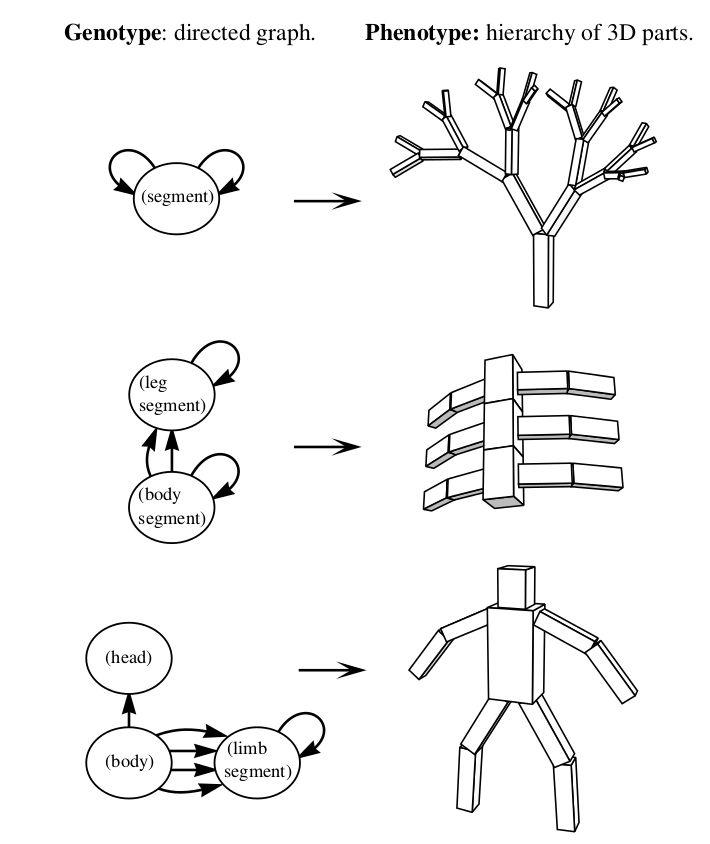
\includegraphics[scale=0.3]{Figures/sims_genotype.png}
    \rule{35em}{0.5pt}
    \caption[Designed examples of genotype graphs and correspond-
    ing creature morphologies.]{Designed examples of genotype graphs and correspond-
    ing creature morphologies.}
    \label{fig:sims_genotype}
\end{figure}

\newpage
Karl Sims uses Genetic Algorithms in order to optimize all the parameters of the control graph and the structure. The mutation and cross-over steps of the Genetic Algorithm have been implemented for updating the population of genotypes. At each evaluation step, creatures are grown from a genotype and compared for a specific task (walking, jumping, swimming). 

\begin{figure}[htbp]
    \centering
    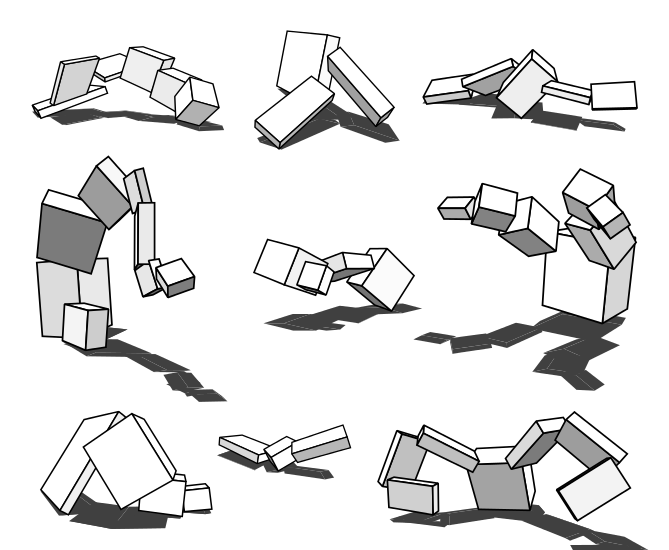
\includegraphics[scale=0.3]{Figures/evolved_creature.png}
    \rule{35em}{0.5pt}
    \caption[Karl Sims Creatures evolved for walking]{Karl Sims Creatures evolved for walking}
    \label{fig:evolved_creature}
\end{figure}


\newpage
\section{Bio-Robotics lab at EPFL}

In the last ten years, the bio-robotics lab of Ecole Polytechnique lauzanne (EPFL) has led breakthrough in modular Robotics, both in the Mechanical design and the control software. 
Central Pattern Generators are a widely use model to create oscillation for problems such as modular Robotics locomotion. In their work Sproewitz et al \cite{sproewitz} focus on online learning parameters fron a Central Pattern Generator (CPG). A CPG is a graph that relates directly to the physical structure in order to generate oscillation (see description in Learning Models). They use a gradient-free downhill method: Powell's method, to learn the parameters of the CPG. In their design CPGs follow the same concept introduced by Karl Sims, where the physical shape is used to produce a similar graph for control purposes. However, for CPGs the neurons are only oscillators. 

\begin{figure}[htbp]
    \centering
    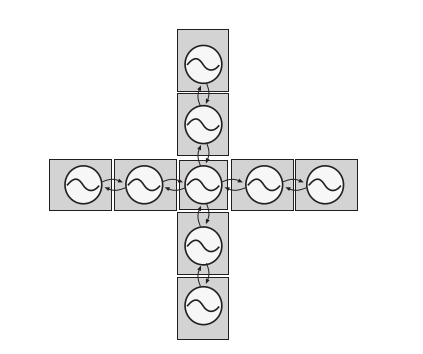
\includegraphics[scale=0.3]{Figures/cpg.png}
    \rule{35em}{0.5pt}
    \caption[Central Pattern Generator Architecture]{Central Pattern Generator Architecture}
    \label{fig:cpg}
\end{figure}

The Bio-Robotics lab also implemented physical blocs in order to build a swarm of modular Robots. The lab produced different prototypes to achieve this goal such as the YaMoR (Yet another Modular Robot) or Roombots module 

\begin{figure}[htbp]
    \centering
    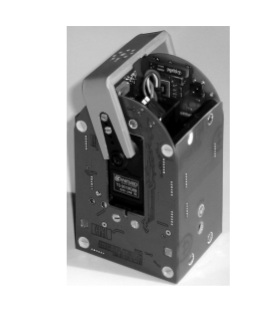
\includegraphics[scale=0.3]{Figures/yamor.png}
    \rule{35em}{0.5pt}
    \caption[Modular Robots implementation]{Modular Robots implementation}
    \label{fig:yamor}
\end{figure}


\section{Flexible Muscle-Based Locomotion for bipedal creatures}

\begin{figure}[htbp]
    \centering
    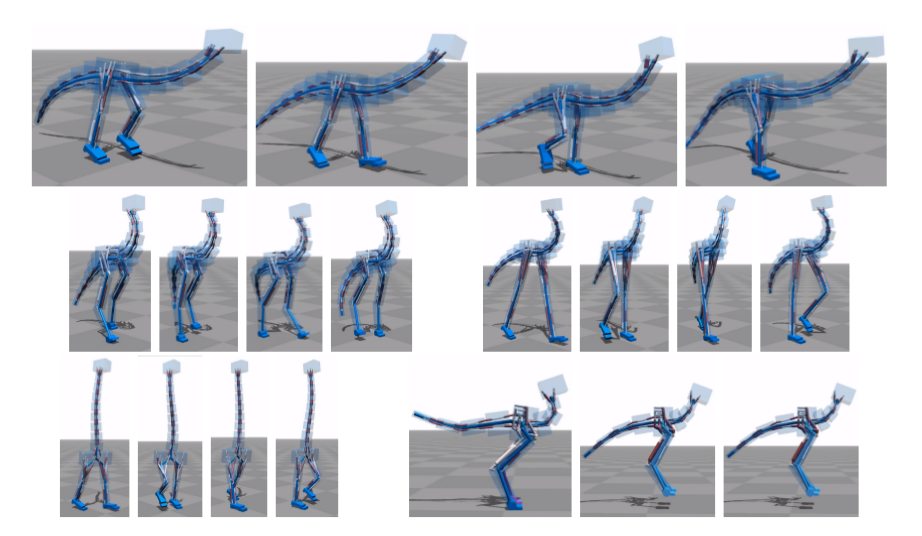
\includegraphics[scale=0.3]{Figures/synthesized_walking.png}
    \rule{35em}{0.5pt}
    \caption[Synthesized walking for a bipedial creature]{Synthesized walking for a bipedal creature}
    \label{fig:yamor}
\end{figure}

More recently, the progress of computational power and the growing interest of building humanoid robots for different tasks in non-friendly environment, such as the initiative from Virginia Tech to build a disaster response robots, or the growing demand of the animation movie and video games industry led to new results. Geijtenbeek et al \cite{MuscleBasedBipeds} used muscle-based actuators and optimize at the same time the routing of the muscles and the control of the muscle activation from a musculoskeletal model. Though this approach is for graphic purposes (SIGGRAPH Conference) and it uses a musculoskeletal model, they follow the same method : a specific control model (simulation of the physical response and interaction of muscles) and a learning algorithm. In this paper, they use covariance matrix adaptation as a the optimization method \cite{igel2007covariance}. This method updates a population of solutions by building new generations at each step based on a normal distribution, which mean and covariance are estimated from the evaluation of the previous generation. Their results showed robust locomotion for different speed, target directions and small ground variations in terrain.

\begin{figure}[htbp]
    \centering
    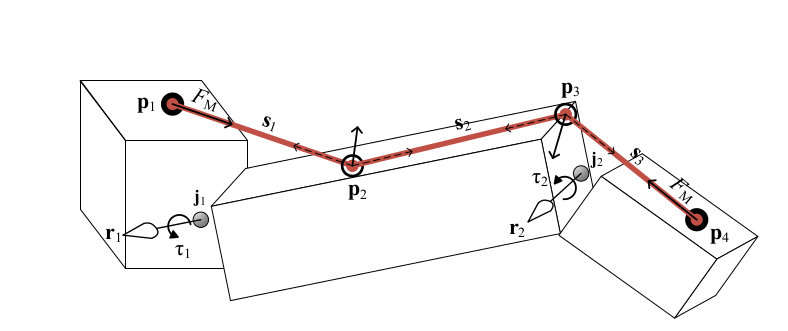
\includegraphics[scale=0.2]{Figures/muscle_based.png}
    \rule{35em}{0.5pt}
    \caption[Example of Muscle Path]{Example of Muscle Path}
    \label{fig:yamor}
\end{figure}


